\doublespacing
\chapter{Experiment}
We describe an application which would benefit from our algorithm, namely RNA secondary structure comparison. 

\section{RNA and its Secondary Structure}
RNA is an essential molecule in organisms which has a wide range of functions in biological systems.Cellular organisms use messenger RNA (mRNA) to convey genetic information (using the letters G, U, A, and C to denote the nitrogenous bases guanine, uracil, adenine, and cytosine) that directs synthesis of specific proteins. Besides, many viruses encode their genetic information using an RNA genome.

RNA is assembled as a chain of nucleotides, but unlike DNA it is more often found in nature as a single-strand folded onto itself, rather than a paired double-strand. However, it can fold back onto itself by means of hydrogen bonding between distant complementary nucleotides(A=U, G$\equiv$C), resulting in the secondary structure. We define the secondary structure of RNA as follows.

\begin{definition}
(RNA secondary structure) A secondary structure is primarily a list of base pair $\omega$. A valid secondary structure should satisfy the following constraints:
\begin{itemize}
\item A base cannot participate in more than one base pair, i.e., $\omega$ is a matching on the set of sequence positions.
\item No two base pairs $(i, j)$ and $(k, l)$ $\in \omega$ "cross" in the sense that $i < k < j < l$.
\end{itemize}
\end{definition}

The first condition excludes tertiary structure motifs such as base triplets while the second condition avoid the pseudo knot in RNA structures. However, the fact is that pseudo knots do occur in RNA structures, namely RNA tertiary structure. To simplify, we don't consider the tertiary structure of RNA in this experiment and assume that any nucleotide participates in at most one such pair and the bonded pairs are non-crossing. 

Figure 5.1 is an example of invalid RNA structure in our experiment, which has tertiary structures(marked in dotted blue lines) and base triplets.
\begin{figure}
		\centering
		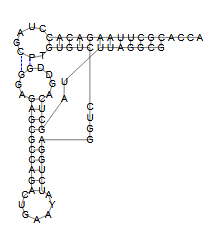
\includegraphics[width=5cm,clip]{Figures/RNATT}
		\label{RNA Tertiary Structure.} 
		\caption{RNA Tertiary Structure.}
\end{figure}
\section{String Representation of the RNA Secondary Structure}
Secondary structure can also been stored compactly in strings consisting of dots and matching brackets:For any pair between positions i and j $(i < j)$ we place an open bracket "(" at position i and a closed bracket ")" at j, while unpaired positions in the molecule are represented by a dot ".".Figure 5.2 illustrates the string presentation with dots and brackets of the RNA secondary structure. 

\begin{figure}
		\centering
		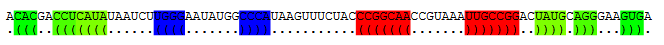
\includegraphics[width=18cm,clip]{Figures/RNAST1}
		\label{String Representation of the RNA Secondary Structure.} 
		\caption{String representation of the RNA secondary structure.}
\end{figure}
\section{RNA Secondary Structure Graphs}
Secondary structures can be represented by "secondary structure graphs". According the base pair information in Figure 5.2, the string can be fold into a circle(Figure 5.3 on the left) or a secondary structure graph(Figure 5.3 on the right).

\begin{figure}
		\centering
		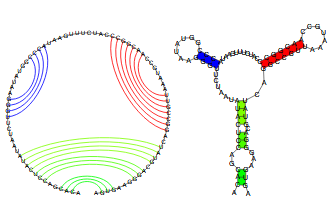
\includegraphics[width=10cm,clip]{Figures/RNAST2}
		\label{Graph Representation of the RNA Secondary Structure.} 
		\caption{Graph representation of the RNA secondary structure.}
\end{figure}

\section{Tree Representation of the RNA Secondary Structure}
In the computer science point of view, the secondary structure of an RNA molecule can be topologically represented by a tree. As shown in Figure 5.2, the RNA secondary structure graphs consists of two distinct category of nucleotides: those that are interacting via hydrogen bonding (so called stems), and those that are not(so call loops). Stems and loops in RNA can be represented as nodes in a tree. Leaves may be labeled with the corresponding unpaired base, while interior nodes are labeled with the corresponding base pair. To make things simplifier, we use different characters apart from alphabet$\{A, U, G, C\}$ to labeled each base pairs. Table 5.1 illustrates the label of each base pairs. 
\begin{table}
			\centering
			\begin{tabular}{l l}
				\toprule
				\textbf{Base Pairs} & \textbf{Label}\\
				\midrule
				$A = U$ & F\\
				$G \equiv C$ & J\\
				$U = A$ & P\\
				$C \equiv G$ & M\\
			\end{tabular}
		\caption{The Label of Base Pair}
\end{table}
In this way,the RNA secondary structure can be converted into a tree. Figure 5.4 is the corresponding tree representation of the secondary structure of RNA in Figure 5.3.

\begin{figure}
		\centering
		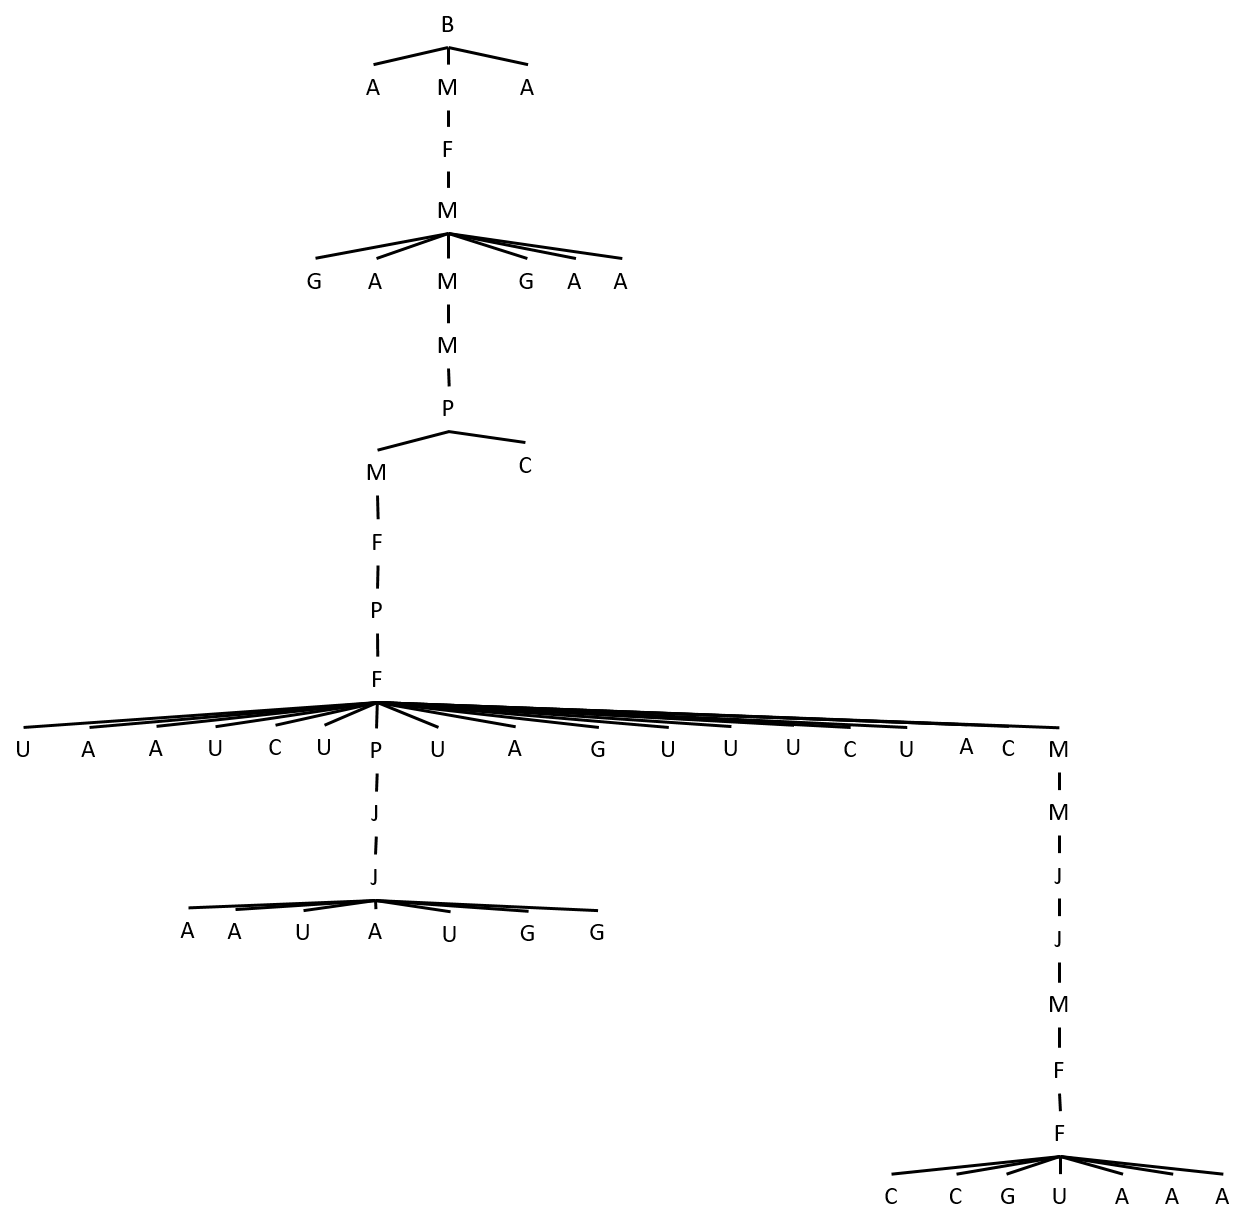
\includegraphics[width=16cm,clip]{Figures/RNAST3}
		\label{Tree Representation of the RNA Secondary Structure.} 
		\caption{Tree representation of the RNA secondary structure.}
\end{figure}

\section{Datasets}
We grab RNA data from the Ribonuclease P Database~\cite{brown1998ribonuclease}. The database consists of a compilation of RNase P sequences, sequence alignments, secondary structures,  three-dimensional models and accessory information as well. The data can be downloaded from the website
\url{http://www.mbio.ncsu.edu/RNaseP/home.html}.

The RNA files in the database are stored in XML format. The RNA files consist of RNA names, description, sequences as well as secondary structure base pairs.
Figure 5.4 is an example of RNA files in the database. The RNA name is "A.tumefaciens RNase P RNA" with the length 402 nt. These two information are included between tags. The following information is the RNA sequence. The RNA second structure information is stored in base pairs indexed by the position in the RNA sequence. Each lines has two base indexes, meaning that two nucleotides are binding to each other. 
\begin{figure}
		\centering
		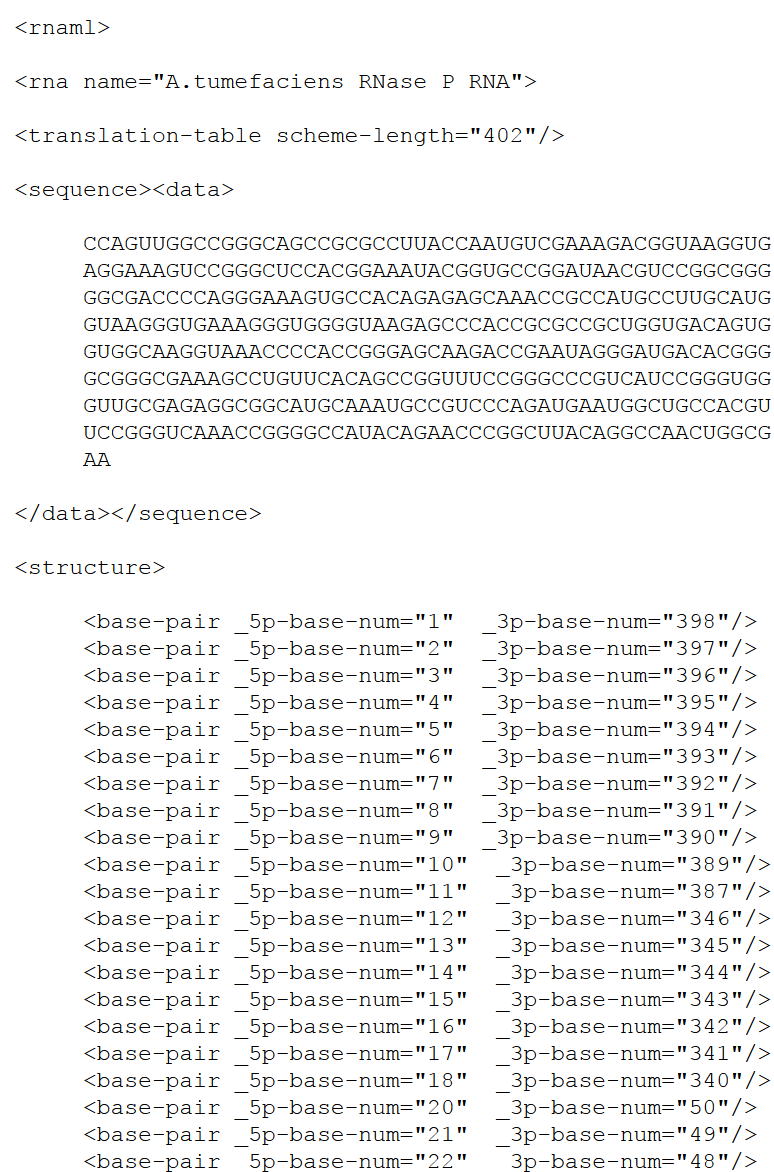
\includegraphics[width=13cm,clip]{Figures/RNADatabase}
		\label{An RNA Sequence in XML Format.} 
		\caption{An RNA Sequence in XML Format.}
\end{figure}

We use the information from RNA files to construct trees. Then the problem of comparing the similarity between two RNA secondary structures becomes comparing the edit distance between two trees. Our algorithms in Chapter 3 and 4 can help solve the problem. 

Another dataset we use in our experiments 

\section{Some Experimental Result}
In our experiments, we compute alignments between RNA secondary structure from Ribonuclease P Database. Figures 5.6 and 5.7 show two RNA structures in string representation. On the other hand, the corresponding graph representations are shown in Figures 5.8 and 5.9. We notice that the raw data contains tertiary structures. Therefore, we first remove the tertiary structures before constructing the corresponding tree data structure. Figure 5.10 shows the alignment results where the cost of each valid operation(deletion, insertion and substitution) is 1.

\begin{figure}
		\centering
		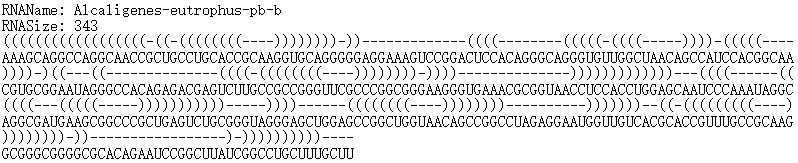
\includegraphics[width=17cm,clip]{Figures/AlcaligenesString}
		\label{Alcaligenes eutrophus Sequence from the RNase P database.} 
		\caption{Alcaligenes eutrophus Sequence from the RNase P database.}
\end{figure}

\begin{figure}
		\centering
		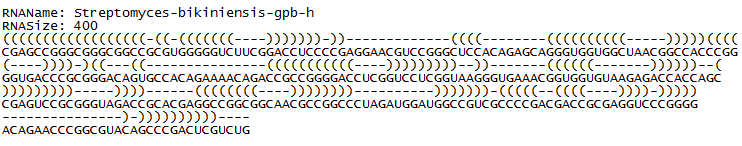
\includegraphics[width=17cm,clip]{Figures/StreptomycesString}
		\label{Streptomyces bikiniensis Sequence from the Rnase P database.} 
		\caption{Streptomyces bikiniensis Sequence from the RNase P database. }
\end{figure} 

\begin{figure}
		\centering
		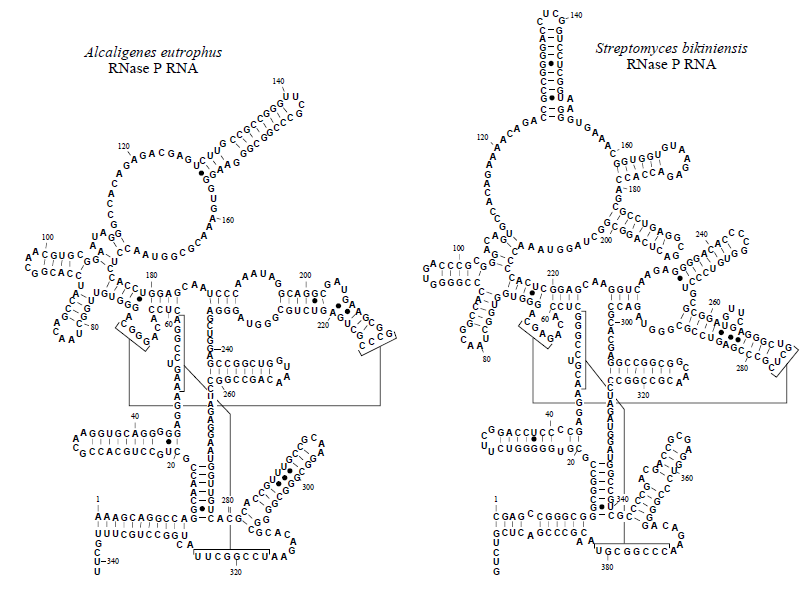
\includegraphics[width=13cm,clip]{Figures/RNAGraphExample}
		\label{The structures of RNase P RNA of Cupriavidus metallidurans (Alcaligenes eutrophus) and Streptomyces bikiniensis.} 
		\caption{The structures of RNase P RNA of Cupriavidus metallidurans (Alcaligenes
eutrophus) and Streptomyces bikiniensis.}
\end{figure}

\begin{figure}
		\centering
		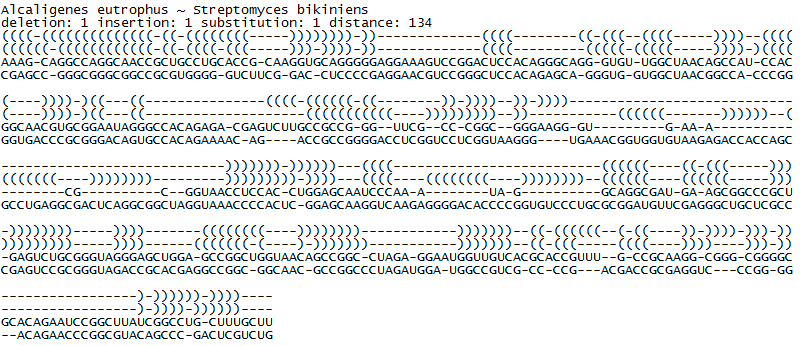
\includegraphics[width=17cm,clip]{Figures/AlignmentResult}
		\label{Alignment Between Two RNAs.} 
		\caption{Alignment Between the Secondary Structure of Alcaligenes eutrophus and Streptomyces bikiniensis.}
\end{figure}

We run our program on larger RNA sequences as well. We compare the edit distance between 2 rRNAs from two organism named "Marchantia polymorpha Chloroplast" and "Archaeoglobus fulgidus". Both of them have the length over 1000 nucleotides. The test result when the cost of each valid operations is 1 is shown in Figure 5.10. 

\section{Evaluation}
We empirically evaluate our algorithm with other four state-of-the-art algorithms on Ribonuclease P Database and compare the relevant sub-problems and actual run time to the algorithms proposed in Chapter 2: the algorithm by Zhang and Shasha and its symmetric version always using right paths~\cite{zhang1989simple}. All algorithms are implemented as single-thread applications in C++ and run on a 64-core 3.4GHZ Ubuntu. The source code is available online.

Firstly we compare the number of relevant sub-problem computed by each of the algorithms for a pair of specific RNA secondary structures. Each relevant sub-problems are the constant-time operations that make up the complexity of the algorithm. Then, we mark the actual run time of each algorithms. The evaluation results are shown in Table 5.2 and 5.3. As according to our test results, our decomposition strategies on compressed trees is the best strategies compared to other methods, creating the least number of relevant sub-problems. 

\begin{table}
			\centering
			\begin{tabular}{l l l}
				\toprule
				\textbf{Algorithm} & \textbf{$\#Rel.sub$} &\textbf{Time[sec]}\\
				\midrule
				$Zhang-L$ & 849282 & 0.08\\
				$Zhang-R$ & 2039089 & 0.13\\
				$Our\ Algorithm(Before\ Compression)$ & 553526 & 0.04\\
				$Zhang-L(Compressed)$ & 428766 & 0.05\\
				$Zhang-R(Compressed)$ & 686562 & 0.05\\
				$Our\ Algorithm(After\ Compression)$ & 291329 & 0.03\\
			\end{tabular}
		\caption{The Relevant Sub-problem and its Actual Run Time of Each Algorithms}
\end{table}

\begin{table}
			\centering
			\begin{tabular}{l l l}
				\toprule
				\textbf{Algorithm} & \textbf{$\#Rel.sub$} &\textbf{Time[sec]}\\
				\midrule
				$Zhang-L$ & 41889364 & 3.2\\
				$Zhang-R$ & 42972591 & 3.3\\
				$Our\ Algorithm(Before\ Compression)$ & 32254346 & 2.3\\
				$Zhang-L(Compressed)$ & 17769036 & 0.47\\
				$Zhang-R(Compressed)$ & 18154025 & 0.51\\
				$Our\ Algorithm(After\ Compression)$ & 13546825 & 0.34\\
			\end{tabular}
		\caption{The Relevant Sub-problem and its Actual Run Time of Each Algorithms}
\end{table}




\begin{figure}
		\centering
		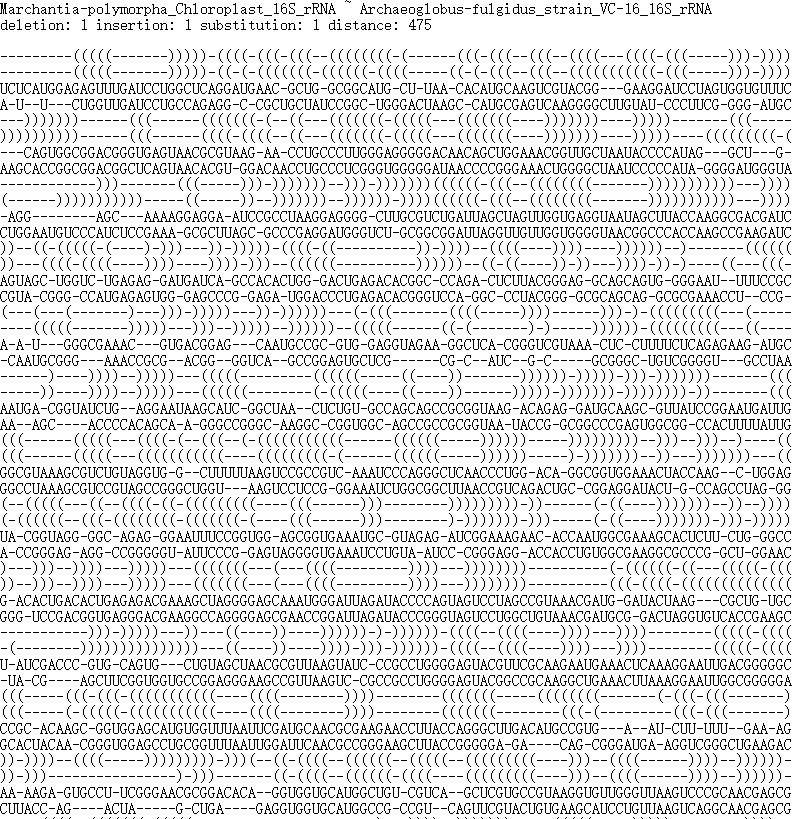
\includegraphics[width=17cm,clip]{Figures/AlignmentResult2}
		\label{Alignment Between Two RNAs.} 
		\caption{Alignment Between the Secondary Structure of rRNA from Marchantia polymorpha Chloroplast and Archaeoglobus fulgidus.}
\end{figure}



